% Created 2017-12-18 lun 14:45
% Intended LaTeX compiler: pdflatex
\documentclass[11pt]{article}
\usepackage[utf8]{inputenc}
\usepackage[T1]{fontenc}
\usepackage{graphicx}
\usepackage{grffile}
\usepackage{longtable}
\usepackage{wrapfig}
\usepackage{rotating}
\usepackage[normalem]{ulem}
\usepackage{amsmath}
\usepackage{textcomp}
\usepackage{amssymb}
\usepackage{capt-of}
\usepackage{hyperref}
\usepackage[margin=3cm]{geometry}
\usepackage{xfrac}
\author{Dean}
\date{\today}
\title{}
\hypersetup{
 pdfauthor={Dean},
 pdftitle={},
 pdfkeywords={},
 pdfsubject={},
 pdfcreator={Emacs 25.3.1 (Org mode 9.1.3)},
 pdflang={English}}
\begin{document}


\section{P1}
\label{sec:orgb29a10e}
\subsection{Metode del trapezi i quadratura de Newton}
\label{sec:org9bb5414}
\subsubsection{Valors obtinguts:}
\label{sec:org37bfd66}
\begin{center}
\begin{tabular}{lrrrrrr}
Subintervals & 4 & 8 & 16 & 32 & 64 & 128\\
Quadratura de Simpson & 0.9878242 & 0.0506787 & 0.1516852 & 0.3574180 & 0.3162449 & 0.3159174\\
Metode del Trapezi & 0.2114939 & -0.4753275 & 0.1954926 & 0.1715777 & 0.3111791 & 0.3149939\\
Subintervals & 256 & 512 & 1024 & 2048 & 4096 & 8192\\
Quadratura de Simpson & 0.3159050 & 0.3159043 & 0.3159042 & 0.3159042 & 0.3159042 & 0.3159042\\
Metode del Trapezi & 0.3156883 & 0.3158510 & 0.3158910 & 0.3159009 & 0.3159034 & 0.3159040\\
\end{tabular}
\end{center}

\begin{figure}[htbp]
\centering
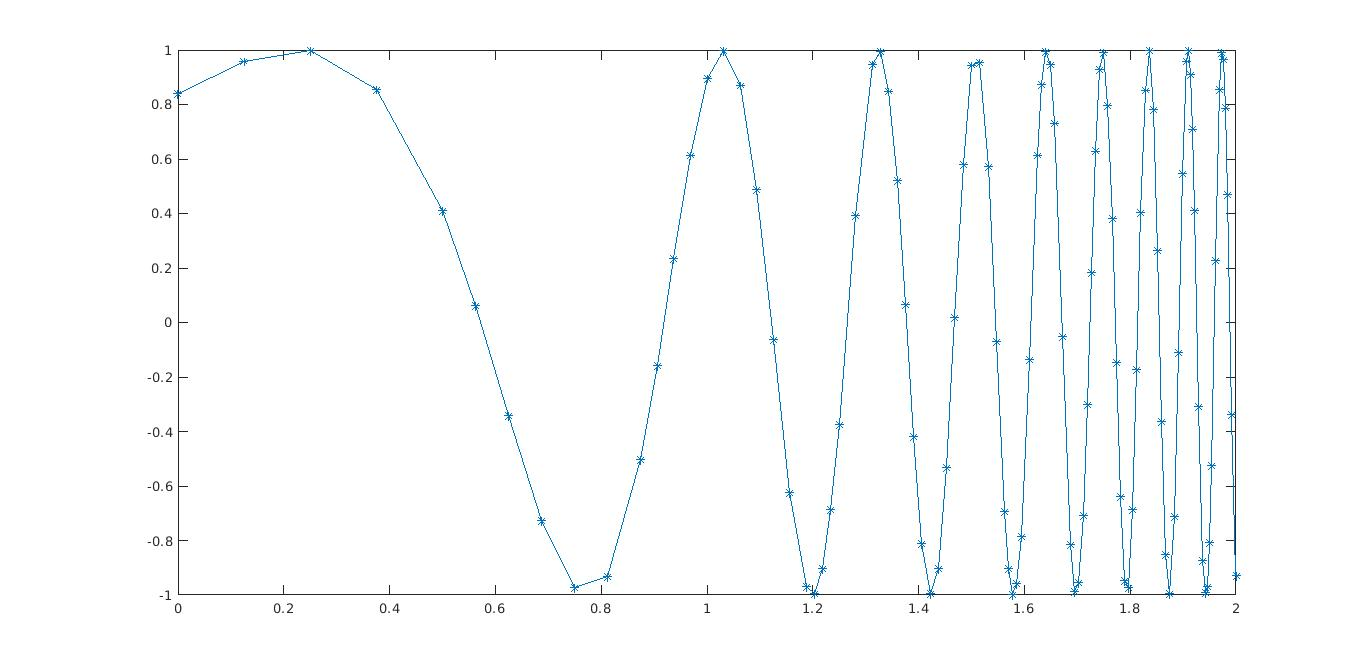
\includegraphics[width=.9\linewidth]{./TrapezivsSimpson.jpg}
\caption{\label{fig:org74d4e06}
Convergencia de les quadratures}
\end{figure}

Observem que ambdos metodes convergeixen correctement, el metode del trapezi te una convergencia quadratica i la quadratura de Simpson una convergencia proporcional a h\(^{\text{5}}\).

Sabent que l'error que comentem a la quadratura de simpson decreix amb un ordre de 5, podem soposar que la longitud per la qual l'error es menor a 10\(^{\text{-6}}\) sera approximadament \#Subintervals = 2/h = \(\frac{2}{^5\sqrt{10^6}}\). Necessitarem aproximadament 32 intervals.
\subsection{Simpson Adaptat}
\label{sec:org43aab63}
\subsubsection{Fita del Error}
\label{sec:org43e0ccb}
Volem veure que la quadratura de Simpson adaptada ens produeix un error fitat (per \(2\epsilon\) en aquest cas). Considerem tots els intervals (x\(_{\text{i}}\), y\(_{\text{i}}\)) tals que retornen el valor de la quadratura sense fer la crida recursiva. Sigui E\(_{\text{i}}\) l'error comes per l'interval i-essim, com tots aquests intervals son disjunts i la seva unio es (0,2) tenim que:
\[ \sum_{i=0}^{r} E_{i} < \sum_{i=0}^{r} (y_i - x_i)*\epsilon = (b-a)*\epsilon = 2\epsilon \]
Per tant l'error esta fitat per \(2\epsilon.\)
\subsubsection{Valors obtinguts}
\label{sec:org0c9c664}
Cridant a la funcio amb una tolerancia de 10\(^{\text{-3}}\) obtenim 0.3159216 i un error absolut de 6.4188e-04. mentres que la funcio \emph{integral} a matlab ens retorna 0.3159042. En efecte, hem comes un error menor a 2\(\cdot\)10\(^{\text{-3}}\).

Els intervals que utilitzem en aquest cas son (200 punts):

\begin{figure}[htbp]
\centering
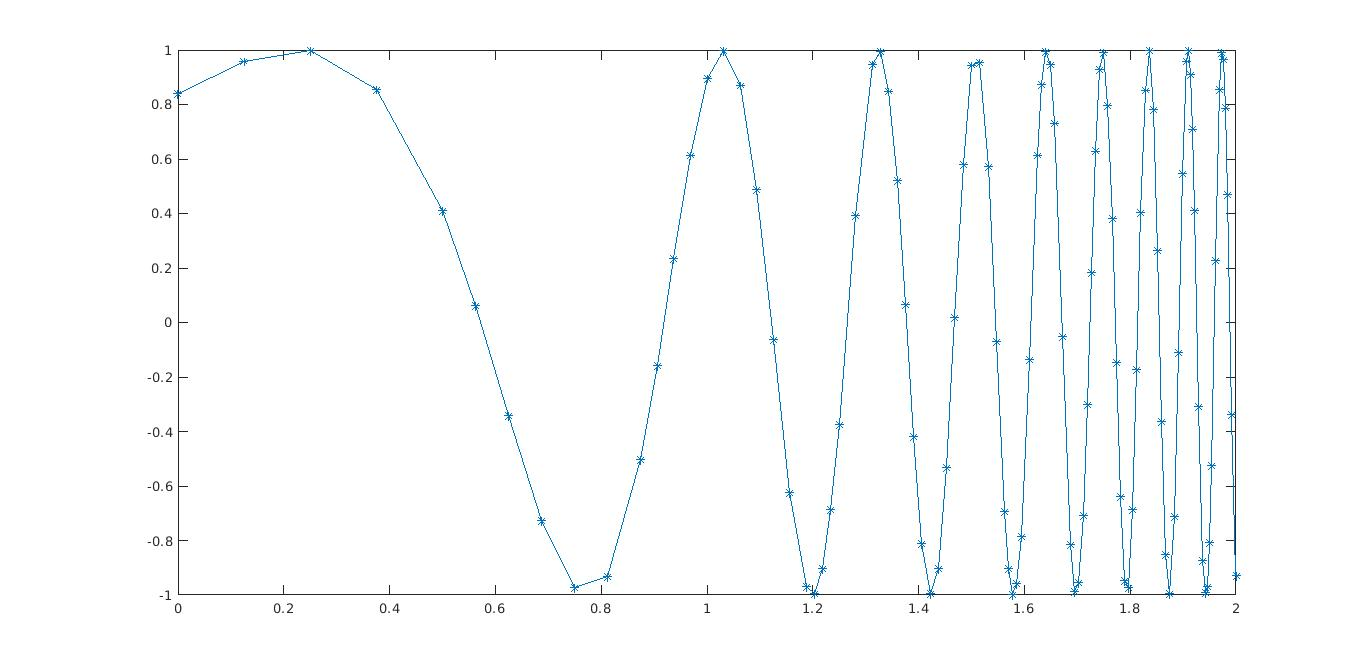
\includegraphics[width=.9\linewidth]{./SimpsonAdaptat.jpg}
\caption{\label{fig:orga5ffe4e}
Simpson Adaptat amb tolerancia 10\(^{\text{-3}}\)}
\end{figure}

Si volem una precisio de 10\(^{\text{-6}}\) obtenim com a resposta 0.3159041 i utilitzem 579 punts:

\begin{figure}[htbp]
\centering
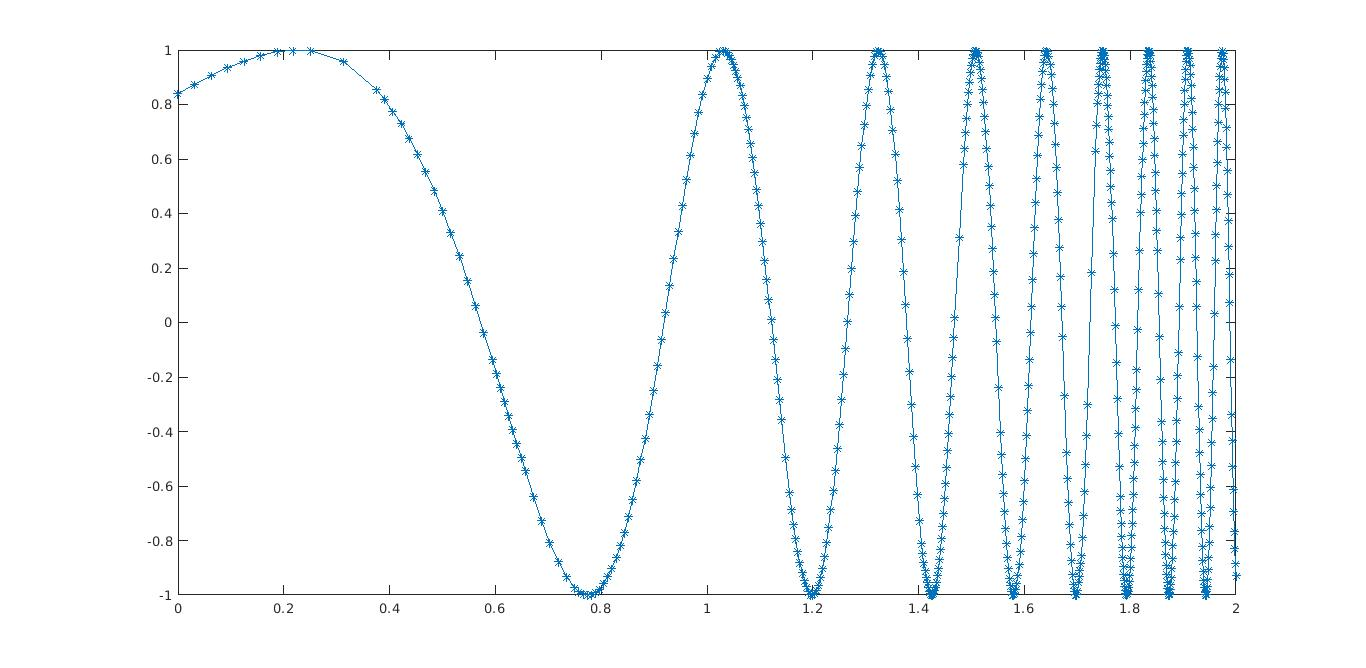
\includegraphics[width=.9\linewidth]{./SimpsonAdaptat2.jpg}
\caption{\label{fig:org2803368}
Simpson Adaptat amb tolerancia 10\(^{\text{-6}}\)}
\end{figure}

Donat que la figura oscil.la molt mes a la esquerre, si utilitzem la quadratura de simpson amb intervals uniformes utilitzem molts mes punts dels que necessitem, ja que a l'interval (0,1) no calen masses punts per poder aproximar el valor de l'integral. La quadratura de Simpson adaptada ens permet aproximar l'integral sense fer servir punts inutils. De fet quan volem una precisio de 10\(^{\text{-6}}\) nomes 68 punts es troben a l'interval (0,1)
\end{document}